\chapter{Background Theory}

  \section{Authentication}

    Authentication is the process of verifying whether a particular individual or a device should be granted access to a system or application running on a device \cite{IPAS}, e.g. verifying that you are the person that you claim to be.

    There are various authentication schemes described in the litterature, but you can broadly group them by the following characteristics \cite{IPAS}:

      \begin{itemize}
        \item Something you know
        \item Something you have, and
        \item Who you are
      \end{itemize}

    ``Something you know'' is often used in the classical login situation where the user have to remember a username/password to get access to a system or device. Some of the commonly used passwords schemes are PIN's, alphanumeric passwords and graphical passwords that all are passwords with the characteristic of ``something you know''.

    In many banking systems you have to use more than just something you know, but also ``something you have'', e.g. a security token, to pass the authentication process. 

    The last characteristic of authentication was ``who you are''. This kind of authentication is called biometric authentication and can be divided into physiological and behavioral characteristics. The first is authentication using unique pcysical charateristics of the user like fingerprints, DNA, iris, etc. The last one are related to the pattern behavior of a person like voice recogition and typing rhythm. 

    Some authentication processes are using more than one of the authentication characteristics to authenticate a user. An example of this is banking systems that often uses ``something you know'' combined with ``something you have''. This is often a username/password and a security token. 

    \subsection{Passwords-based Authentication}

      \subsection*{PIN's}
        Personal identification number is a numeric passwords. The PIN was first introduced in the first ATM in London in 1967 as a efficient way for the banks to authenticate their customers \cite{Bonneau1}.      

      \subsection*{Alphanumeric passwords}

        The word ``Alphanumeric'' is a composiption of the words ``alpha'' (as in alphabet), and ``numeric''(as in numbers). The alphanumeric password may also contain special characters, so in short a alphanumeric password is a mix of all writeable characters.

      \subsection*{Graphical passwords}

      A varity of graphical passwords schemes have been created over the past years. Biddle et al. have collected research of the past decade on graphical password schemes \cite{Biddle}, dividing the schemes into three categories: 

      \begin{itemize}
        \item Recall-based authentication
        \item Recognition-based authentication, and 
        \item Cued-recall authentication.
      \end{itemize}

      {\Large \bf Recall-based} \\
      
      Recall-based graphical passwords are often referred to as drawmetric systems \cite{DeAngeli} because the user are are reproducing a secret drawing. The password is normally drawn in a grid or a blank canvas, requireing the user to reproduce the secret password from its memory. Some of the known recall-based password schemes are Pass-Go and Draw-a-secret (DAS).

        \begin{figure}[H]
          \centering
          \subfigure{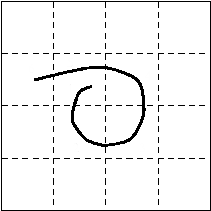
\includegraphics[scale=0.70]{pics/DAS.png}}
          \subfigure{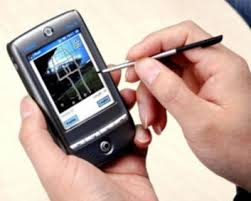
\includegraphics[scale=0.73]{pics/BDAS.jpg}}
          \caption{1) DAS 2)DAS with background}
        \end{figure}

      {\Large \bf Recognition-based}
      
      Recognition-based passwords are often referred to as cognometric systems \cite{DeAngeli} because the user recall a scret drawing, or sequence of drawings, and the reproduces it as the secret password. Example of implemented recognition-based password schemes are `Passface' and `Deja vu' that uses a sequence of user selected faces/images as a authentication code.

        \begin{figure}[H]
          \centering
          \subfigure{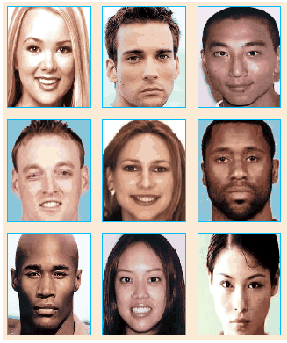
\includegraphics[scale=0.49]{pics/Passface.png}}
          \subfigure{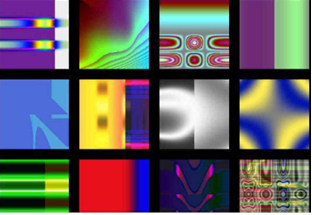
\includegraphics[scale=0.77]{pics/DejaVu.png}}
          \caption{1) Passface 2) Deja vu}
        \end{figure}

      {\Large \bf Cued-recall} \\
      Cued-recall are often referred to locimetric systems \cite{DeAngeli}. With cued-recall authentication typically require the users to remember and target a specific location within and image. This is a version of a recall-based authentication, but helps the user with the recall by showing an image and not just an grid or canvas. It is allso different from the recognition-based approah becuase the user need to indentify spesific locations in an image as a whole. One of the known Cued-Recall password scheme are PassPoints.

        \begin{figure}[H]
          \centering
          \subfigure{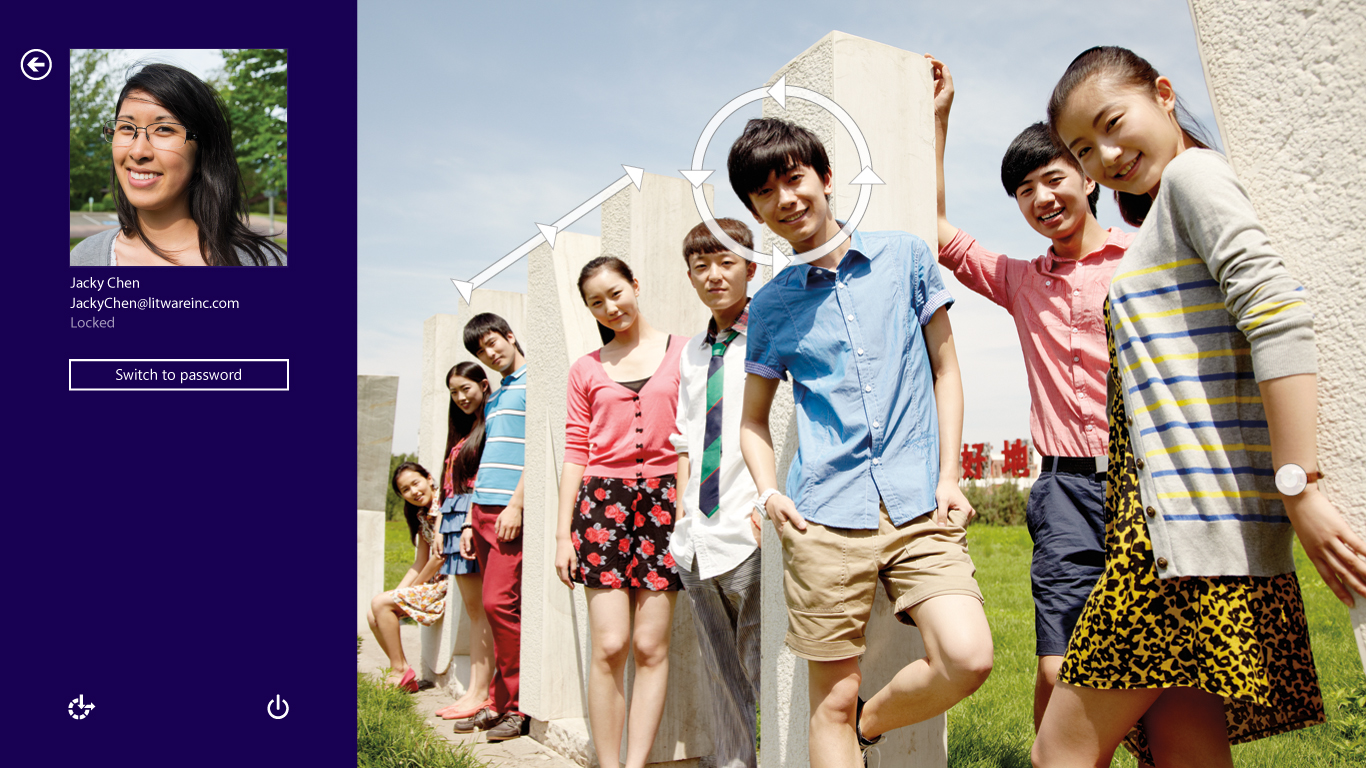
\includegraphics[scale=0.24]{pics/Passpoint.jpg}}
          \caption{1) Passpoints}
        \end{figure}

    \subsection{Token-based Authentication}
      In a token-based authentication process the user uses a security token, that often may be a physical device.
      
    \subsection{Biometrical Authentication}
      Biometric authentication refers to verify a persons identity based on physical or behaviroal characteristics of an individual such as face,fingerprint, hand geometry, iris, keystroke, signature, voice,etc\cite{biometrics, biometrics2}. Biometric authentication are different than other authentications schemes because:

        \begin{itemize}
          \item the biometric password cannot be lost nor forgotten
          \item biometrical passwords tends to be difficult to copy, share and distribute, and 
          \item the person being authenticated needs to be present in the authentication process
        \end{itemize} 

      \subsection*{Physiological Biometrics}
        Physiological biometrics uses the physiological characterisstics of an individual in the authentication process. The verification uses unique characteristics of a human, e.g. physical parts of the body that are unique. Examples of physiological biometrics are fingerprints, face recognition, iris, hand and finger geometry, and DNA. 

      \subsection*{Behavioral Biometrics}

        Behavioral biometrics analyze how a person performs different activities, e.g. applies pattern recognition techniques for activities like keyboard writing, talking and hanDwriting. Examples of behavioral biometrics ae keystroke recognition, voice recognition, and signature recognition. 

    \subsection{Multi-factor Authentication}

  \section{Mobile Security}



 %  \section{Passphrase and PIN's vs. graphical passwords}
 %  \section{A password are more then just a password}

 %    If you take a walk in the street and ask a random person ``what is a password?'', 
 %    you probably get the aswer ``its letters and digits''. Passwords are so much more than just letter and digits. 

 %    Nowadays everything we do require you to keep this secret called a password. Your work, you're social life, 
 %    even you're private life is forcing you to keep track of passwords. How do you keep track of all of them?
 %    You probably keep the same password at many places. 
 %    \subsection{Theoretical Password Space}
 %    \subsection{Practical Password Space}

 %  \section{Relevant Data Collection Methods}
 %    In this section I will explore different methods for collecting data. It will give a brief summary of the 
 %    method as well as summary and discussion of the different methods at the end. 
 %    \subsection{Android Unlock Patterns Games}
 %    \subsection{Relevant User Studies}
 %    \subsection{Summary of Methods}
 %  \section{Information gathering}
	% \section{Psycology and passwords}
	% \section{Graphical passwords}
	% \section{Android Unlock Pattern}
